%%% Local Variables:
%%% mode: latex
%%% TeX-master: "../frankfurt"
%%% End:

\subsection{}
\begin{frame}
\frametitle{Motivation}


\only<1>{


}

\only<2>{


}


\end{frame}


\begin{frame}
  \frametitle{Food Tour Example}

\only<1>{
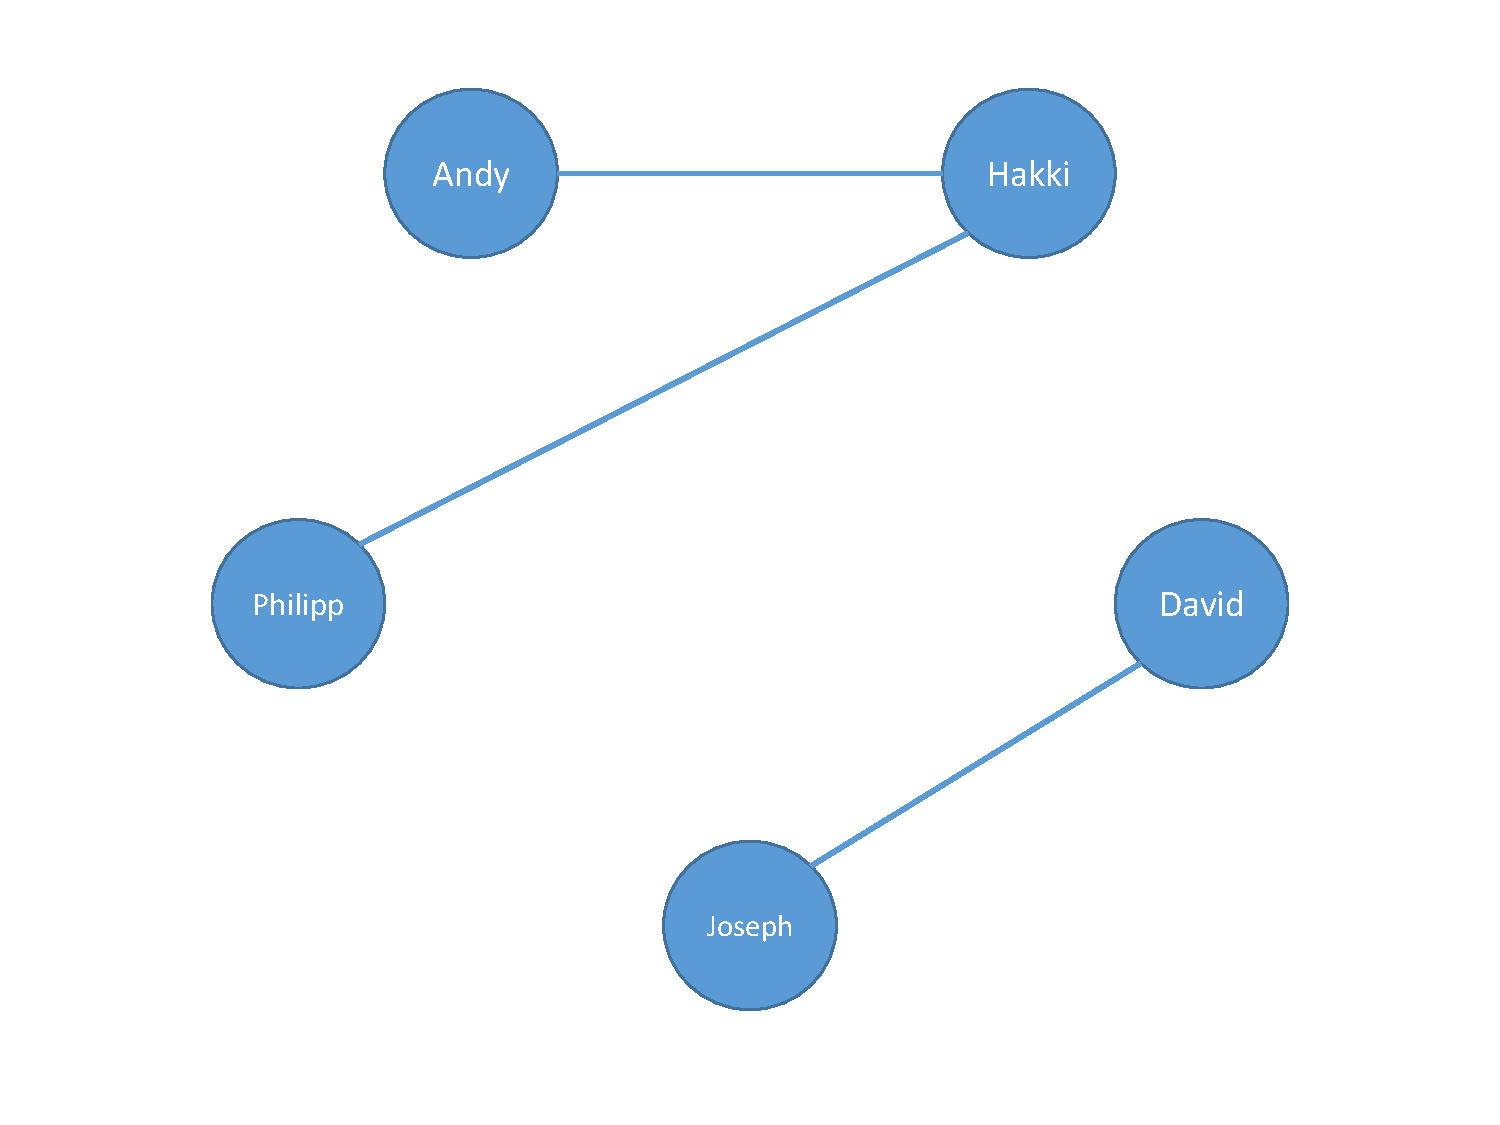
\includegraphics[scale=0.3]{img/foodprefs1.pdf}
}
\only<2>{
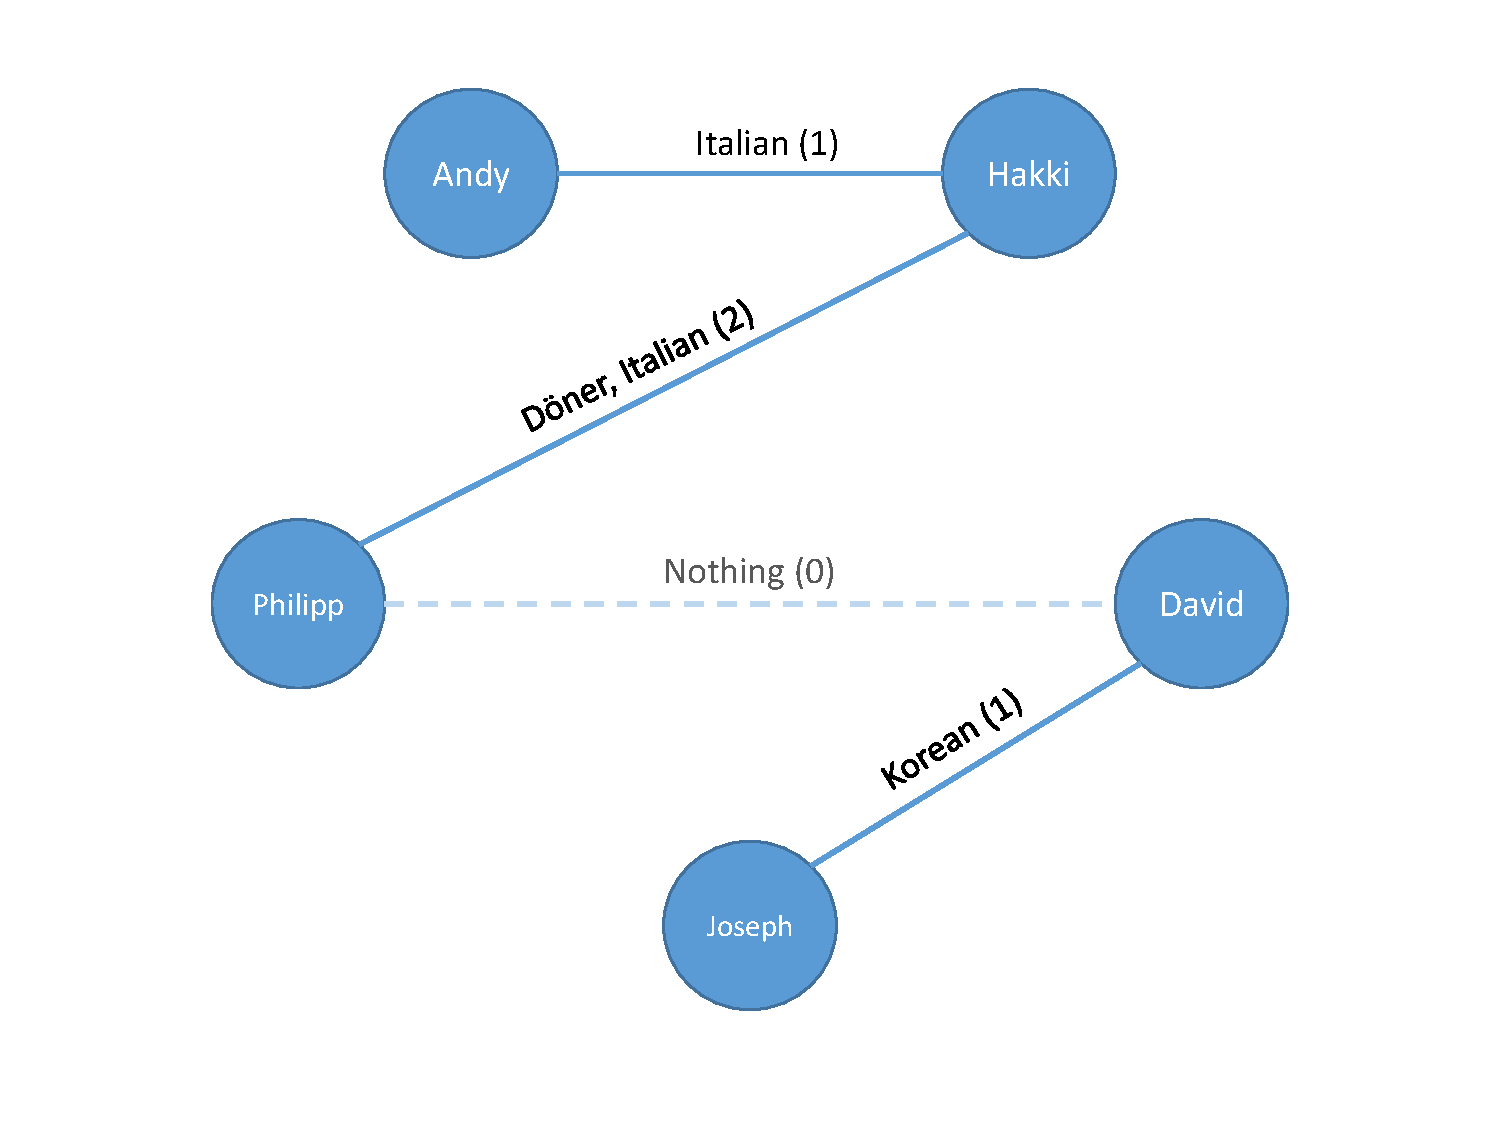
\includegraphics[scale=0.3]{img/foodprefs2.pdf}
}
\only<3>{
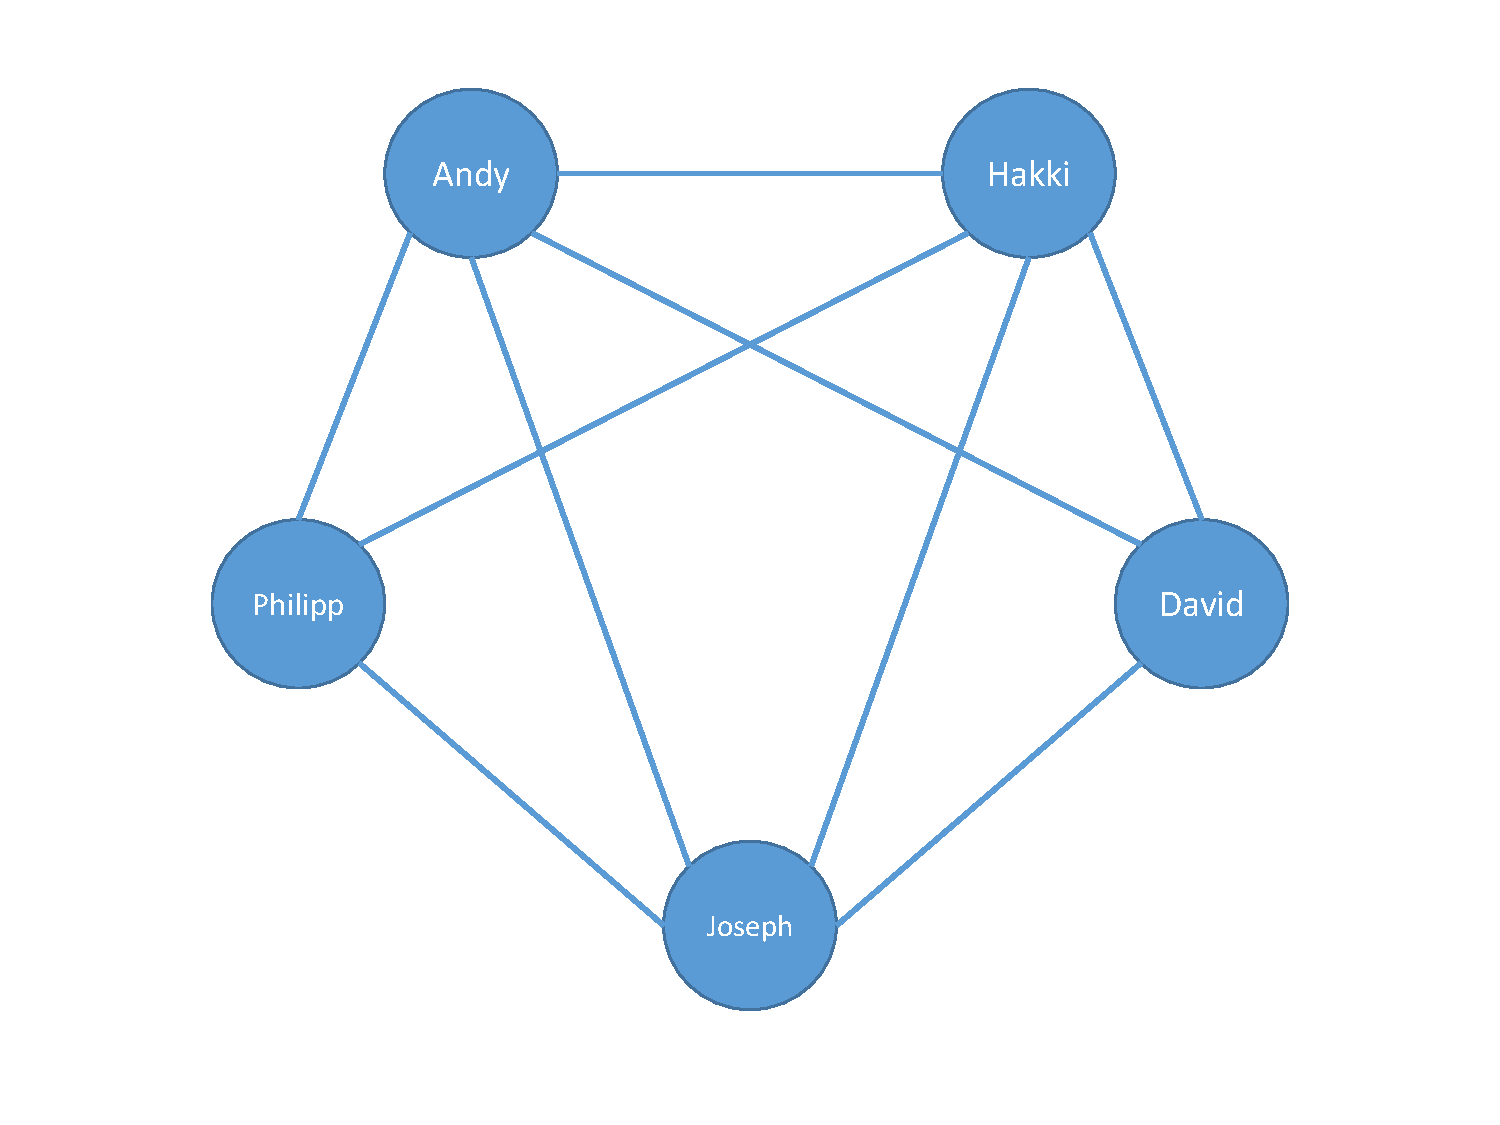
\includegraphics[scale=0.3]{img/foodprefs3.pdf}
}

\end{frame}

\begin{frame}
  \frametitle{Definition}

\only<1>{
  \begin{block}{Cut}
    \begin{itemize}
    \item Undirected graph $G = (V, E)$, $n = \norm{V}$, $m =
      \norm{E}$
    \item Cut problems can be described as partitioning $V$ in to $S$
      and $\overline{S}$, where $S \subset V$:
      \begin{greenblock}{Description}
        \begin{itemize}
        \item Alternatively, finding a subset of $E$ that, if
          removed, splits the graph into two connected componants.
        \item Weight: number of edges between $S$ and $\overline{S}$:
          $$w(S, \overline{S}) = \norm{\{u, v\}\in E ~| ~u \in S \wedge
            v \in \overline{S}}$$
        \end{itemize}
      \end{greenblock}

    \end{itemize}
  \end{block}
}

\only<2>{
  \begin{block}{Min-Cut}
    A cut with minimum weight and $S, \overline{S}
          \ne \phi$

  \end{block}

  \begin{greenblock}{Other Cut Problems}
    \begin{itemize}
    \item Directed Cut: Given $s, t\in V$,ensure $s\in S \wedge t\in
      \overline{S}$;
    \item K-Cut: Cuts the graph into k connected componants;
    \item Sparsest Cut: The sparsest cut problem is to bipartition the vertices so as to minimize the ratio of the number of edges across the cut divided by the number of vertices in the smaller half of the partition.
    \end{itemize}
  \end{greenblock}


}
\end{frame}


\begin{frame}
  \frametitle{Generalization}
  \begin{block}{Difficulty of Cuts}
    Minimum cut can be considered as a subset of $k-cut$ where $k$ is
    a fixed number 2.
    \begin{itemize}
    \item $k-cut$ is $NP-Complete$ problem if $k$ is part of the
      input.
    \item Minimum cut is polynomial time calculable.
    \end{itemize}
  \end{block}

Add anything here?
\end{frame}
